\chapter{Results}
The HLS flow was tested using four distinct functions that make use of different aspects of the supported subset of the Julia language. The following chapter details these functions, the results of their input into the flow, and the observations from simulating the resultant hardware.

\pagebreak

\section{Testbench}
The testbench was used to verify functional correctness of the hardware. This simplified the requirements as the testbench could drive the input signals and check the next valid output. Each testbench was constructed as in Figure \ref{fig:gen_tb} (a full testbench example is in Appendix \ref{app:tb_eg}). 

The testbench contains a verilog function that implements a version of the Julia source function written in verilog. This models the expected result of the hardware and can be directly compared to verify the functional correctness. Random inputs are generated and fed into the Design Under Test (DUT) and the function model. To drive the DUT, the input data signals and the start valid signal need to be asserted and held for two cycles. The hardware will then operate without further input and trigger the end ready signal when the output data is stable and can be read. The number of cycles required to run the hardware is dependent on the control flow so the testbench waits until the end ready signal is asserted before reading the end data value. The result of the comparison generates a fail flag if the DUT output does not match the expected output. This is noted in the simulation logs. If the test passes with no fails then the test registers success.

\begin{figure}[htb!]
    \centering
    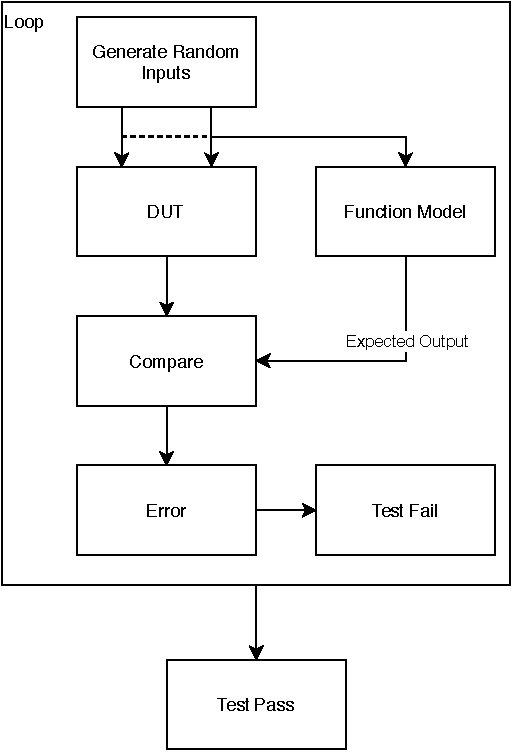
\includegraphics[width=0.5\textwidth]{Images/generic_tb.pdf}
    \caption{Generalised layout for the testbenches used to verify the test functions in simulation}
    \label{fig:gen_tb}
\end{figure}

\pagebreak

\section{\code{mul} function}
\label{sec:mul}

\begin{lstlisting}[
    caption={Three argument, inline multiply function for integers.},
    captionpos=b, 
    label={code:mul_func}
]
mul(a::Integer, b::Integer, c::Integer) = a*b*c
\end{lstlisting}

The \code{mul} function tests the basic aspects of the HLS flow. During the first simulation of the testbench and DUT, there was a compilation error in the generated VHDL. The error occured because the \code{end\_0} component was missing connections on two of the ports. To check where the issue was within the flow, the same \code{mul} function was put through the dynamatic library flow. This yielded the same DOT graph and therefore the same VHDL as both flows use the same VHDL converter. This was an unexpected error in the VHDL converter causing the issue. Upon closer inspection of the signal related to the testbench error, it was noticed that making a small manual change to the VHDL prevented the error. The port connection was tied off with a new signal that was not connected to the rest of the hardware. This is not a failure of the dynamic scheduling package and the slightly edited VHDL was verified to be functionally correct. The manual change does not affect the circuit operation so the result is valid.

\begin{figure}[htb!]
    \centering
    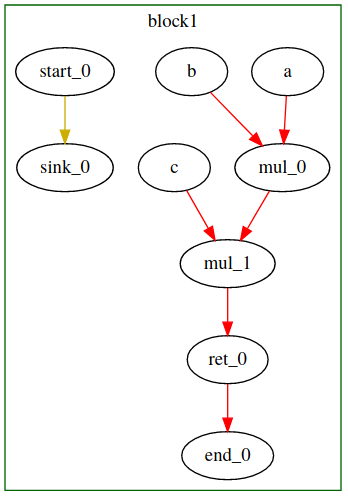
\includegraphics[width=0.4\textwidth]{Images/mul_dot.png}
    \caption{Graphical representation of the dynamic scheduling result for the \code{mul} function. This was directly generated from the DOT graph output using a browser-based graph visualiser \cite{graphviz}.}
    \label{fig:mul_dot}
\end{figure}

\pagebreak

\section{\code{if\_else} function}
\label{sec:ie}

\begin{lstlisting}[
    caption={A simple test function with a branching control flow.},
    captionpos=b, 
    label={code:ie_func}
]
function if_else(a::Integer, b::Integer)
        k = a - b;
        if a > b
                k = k * a
                return k
        elseif b > a
                k = k * b
                return k
        else
                return k
        end
end
\end{lstlisting}

The \code{if\_else} function was chosen to test the implementation of the basics of the branching pass in the dynamic scheduling package. Figure \ref{fig:ie_dot} shows the visual representation of dynamically scheduled circuit. The first set of testing would enter a dead state in which no result would appear at the output. This was due to a minor bug in the branch pass. The bug caused the data flow of the \code{branch\_5} to be driven into the sink state meaning that the valid/ready signal never reached the end node. The bug was fixed to make sure that all branches were connected according to the basic block number rather than the order of successor basic blocks. The VHDL was regnerated with the fix and the testbench was successfully run, verifying the basic branching.

\pagebreak

\begin{figure}[htb!]
    \centering
    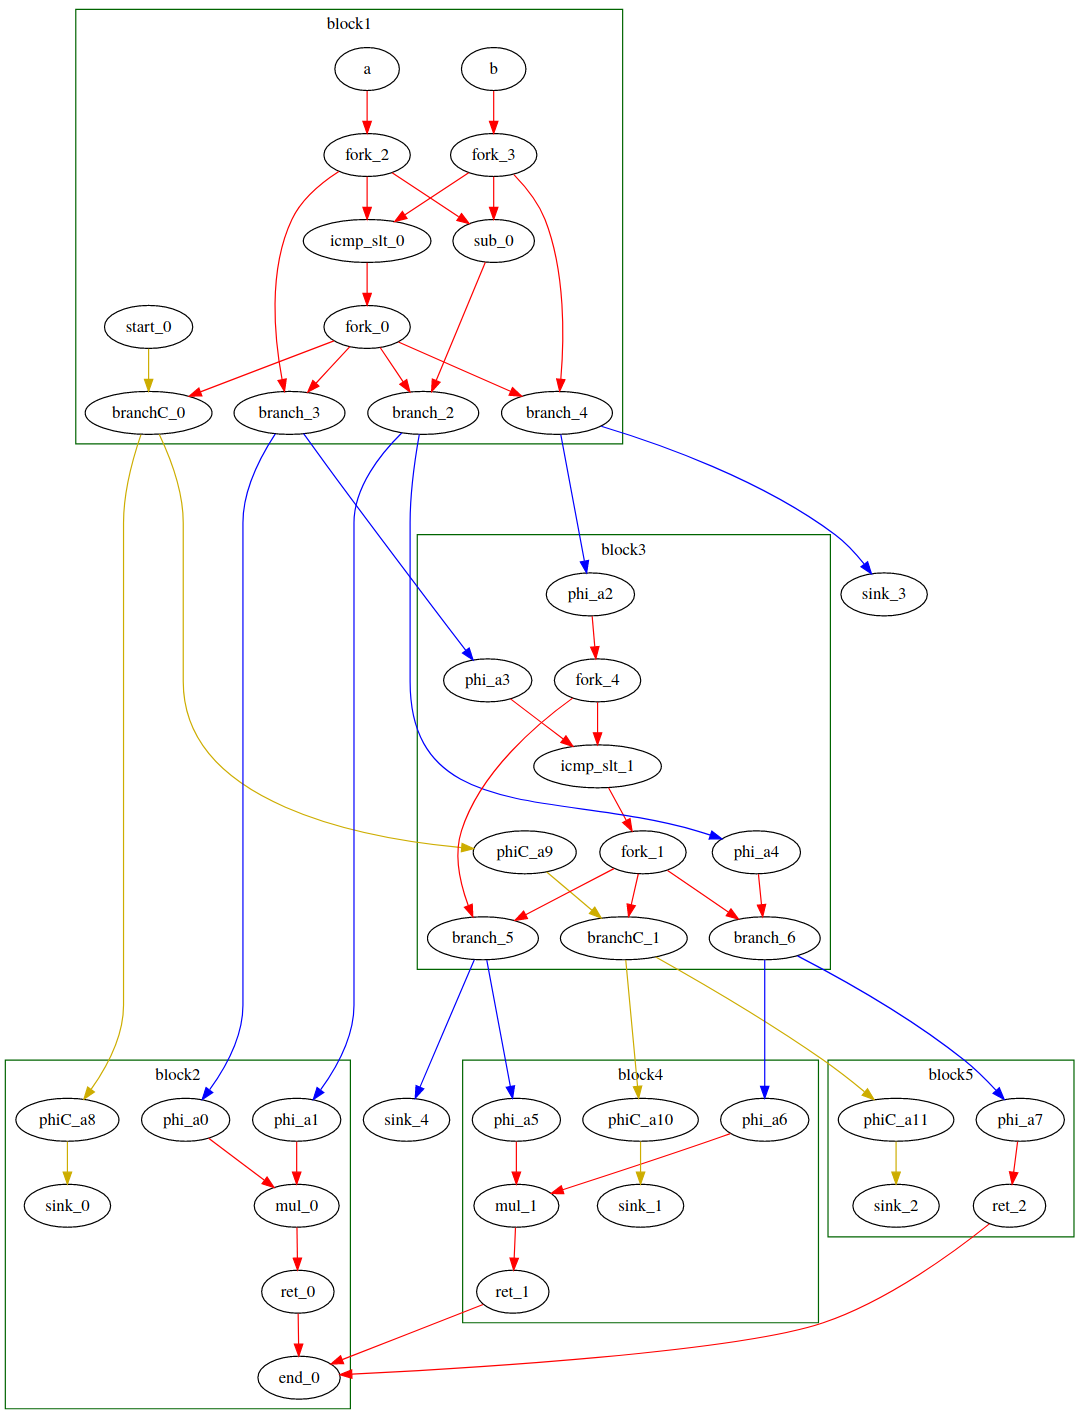
\includegraphics[width=\textwidth]{Images/ie_dot.png}
    \caption{Graphical representation of the dynamic scheduling result for the \code{if\_else} function from Code Snippet \ref{code:ie_func}.}
    \label{fig:ie_dot}
\end{figure}

\pagebreak

\section{looping \code{power} function}
\label{sec:pow}

\begin{lstlisting}[
    caption={Test function to calculate the power using a loop.},
    captionpos=b, 
    label={code:jpow_func}
]
function jpow(x::Int32, n::Int32) #basic power function
        r = Int32(1)
        while n > Int32(0)
                n -= Int32(1)
                r *= x
        end
        return r
end
\end{lstlisting}

The \code{power} function was chosen as it makes use of a while loop. This loop can be seen in Figure \ref{fig:jpow_dot} in the control flow (gold connections) that link BB2 to BB3 and BB3 back to BB2. At the head of the loop are the \code{phi} nodes. These are multiplexers which select the branch input based on the green connection from the \code{phiMC\_} (merge controller). The graph demonstrates that buffer functions have been added in the correct positions within the loop to prevent deadlock.

The inital DOT graph produced used the \code{power} function from Code Snippet \ref{code:jpow}. The difference being the specification of the constant types. The Julia compiler defaults to using 64 bit integers inspite of type inference specifying the method be used for 32 bit integers. This introduces signed extension functions. The dynamatic components do not support 64 bit operations at the time of writing so the decision was made to use 32 bit input types and manually change the constant types.

When running the testbench driven simulation, the random inputs were constrained to being greater than zero as the source function does not produce the correct result given a negative exponent. The generated VHDL was shown to be functionally correct and with each result being returned after $n$ cycles, where $n$ is the randomly generated exponent.

\pagebreak

\begin{figure}[H]
    \centering
    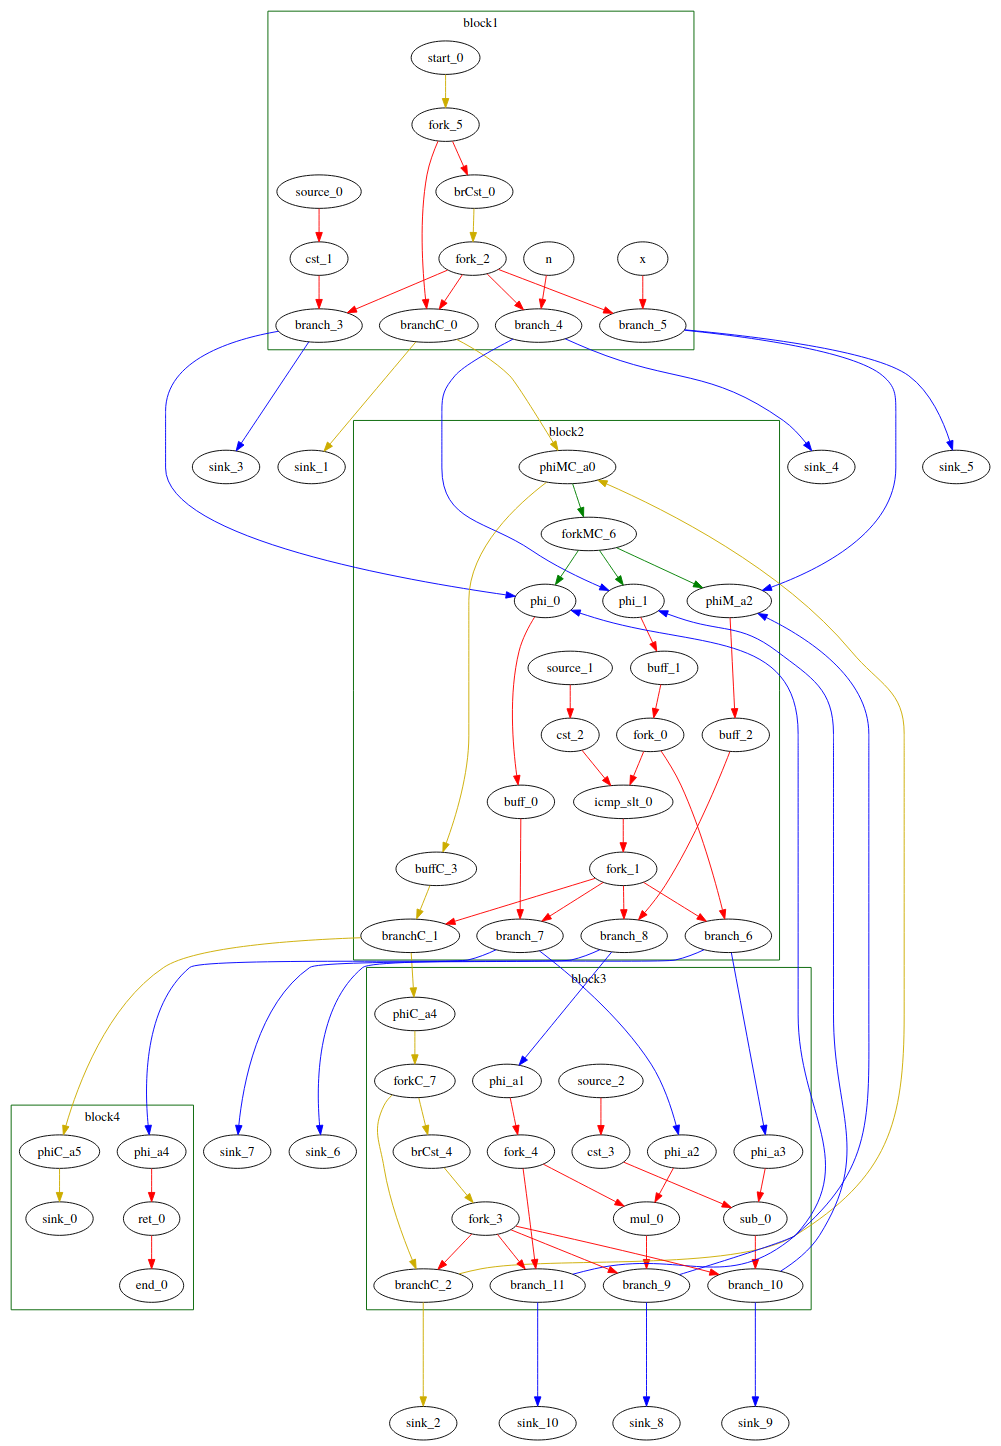
\includegraphics[width=\textwidth]{Images/pow_dot.png}
    \caption{Graphical representation of the dynamic scheduling result for the \code{jpow} function from Code Snippet \ref{code:jpow_func}.}
    \label{fig:jpow_dot}
\end{figure}

\pagebreak

\section{\code{newton\_raphson} function}
\label{sec:nr}

\begin{lstlisting}[
    caption={A more complex function with a branching control flow and looping.},
    captionpos=b, 
    label={code:nr_func}
]
function newton_raphson(rts::Int32, x1::Int32, xh::Int32)
    i = Int32(0)
    dx = Int32(0)

    while i < Int32(300)
            df = Int32(4) * rts;
            f = Int32(2) * rts * rts - Int32(100)
            i+= Int32(1)
            if f < Int32(0)
                    x1 = rts
            else
                    xh = rts
            end

            if ((rts - x1) * df - f) * ((rts - xh) * df - f) <= Int32(0)
                    dx = (xh - x1) \div Int32(2)
                    rts = x1 + dx
            else
                    dx = rts \div Int32(4)
                    rts -= dx
            end
    end
    return rts
end
\end{lstlisting}

The final test function used to determine approximations of roots of the equation $2x^2 - 100$ provided the inputs are near the roots. This usefulness of this version is limited by the use of integer methods. For testing purposes, the function displays more complex branching conditional statements within a loop. The graphical representation have been excluded for brevity. 

%TODO check this number
The generated hardware made use of 225 elastic components including integer multiplication, addition, subtraction, division and comparisons. The first testbench run returned the incorrect value of zero for all inputs, by going through the waveforms of the simulation it was observed that the integer division function was not generating any results. A further look at the compilation transcript showed that, while the connection to the elastic component wrapper was correct, the internal component was not connected. The internal component was part of the proprietary Vivado library that needed to be generated and included in compilation. Once this was added, the generated hardware functioned correctly.

\pagebreak

\section{Synthesis Results}

\begingroup
%\setlength{\tabcolsep}{10pt} % Default value: 6pt
\renewcommand{\arraystretch}{1.5} % Default value: 1

\begin{table}[htb!]
\begin{tabular}{c|cc|cc|cc|cc|cc}
\multirow{2}{*}{Program} & \multicolumn{2}{c|}{Basic Blocks} & \multicolumn{2}{c|}{Components} & \multicolumn{2}{c|}{LUTs} & \multicolumn{2}{c|}{FFs} & \multicolumn{2}{c}{DSPs} \\
                         & Julia            & C++            & Julia           & C++           & Julia        & C++        & Julia        & C++       & Julia        & C++       \\ \hline
\code{mul}                      & 1                & 1              & 9               & 9             & 82           & 82         & 296          & 296       & 6            & 6         \\
\code{if\_else}                 & 5                & 3              & 41              & 32            & 511          & 399        & 595          & 460       & 6            & 6         \\
\code{power}                    & 4                & 4              & 61              & 64            & 555          & 571        & 671          & 710       & 3            & 3         \\
\code{newton\_raphson}          & 10               & 6              & 225             & 147           & 4006         & 3319       & 3456         & 118       & 18           & 12       
\end{tabular}
\caption{Area results of the synthesis of test functions for the Julia Dynamic Scheduling compared to C++ dynamatic flow.}
\label{tab:synth}
\end{table}

\endgroup

The test functions were put through the Julia HLS Flow and the Dynamatic Flow to compare the implementations of dynamic scheduling. During the flow process, some errors were discovered in the Dynamatic output. The stage producing DOT graphs did not provide argument names for the function resulting in the data flow entry components being connected together, preventing the dot2vhdl tool from running initially. The names were added and the tool then proceeded to function correctly. The unused memory interface signals were not automatically generated by the dot2vhdl converter meaning they had to be manually added, as with the Julia Flow. The final issue was with a mismatched connection size within the component definitions. A fork component was connected to the output of a boolean comparison function. The comparison only has a single bit output but the fork was expecting a 32 bit input. This was corrected in the dot file by reducing the fork size to 1 bit to match the comparison, the successor connections of the fork were already configured for single bit inputs so this resolved issues with the hardware. After these changes were made, the designs were verified using the same testbenches as the Julia test functions to make sure the hardware was functionally correct. The resulting VDHL hardware files were then synthesised using Vivado Design Suite version 2018.1 \cite{viv_prod}, following the procedure laid out in the synthesis guide \cite{viv_guide}.

The results from Table \ref{tab:synth} show that the flows produce comparable hardware in the first three test functions with respect to resource usage. The \code{newton\_raphson} test function had a significantly higher resource usage in the Julia Flow as opposed to the Dynamatic Flow. This can mostly be attributed to the number of basic blocks in the program flow. A greater number of basic blocks means an increased number of \code{branch}, \code{merge\_data}, and their associated control components. A less complex control flow is also more likely to contain closely associated data flow components, reducing the number of branch-merge\_data chains implemented to connected components across basic blocks. The Julia typed IR generated for \code{newton\_raphson} contained ten basic blocks and the initial LLVM representation generated by the Clang compiler contained also contained ten blocks. The Dynamatic Flow then runs a series of LLVM passes that result in a simplified CFG, reducing the number of basic blocks to six before dynamic scheduling. There was also a discrepancy in the number of Discrete Signal Processing (DSP) blocks. These blocks are responsible for the multiplication in the \code{mul\_op} components of the circuit. The LLVM passes were responsible for reducing the number of multiplications in the program. The poor results were due to a lack of CDFG optimisation on the part of the SSATools package. %Passes similar to the LLVM CFG simplification pass should be added in future work.

The small reduction in resources in the \code{power} was due to the differing implementations of the cycle pass and simple buffer pass in the Julia Flow and Dynamatic Flow respectively. While this saved the implementation a some buffer components in the short term, the Dynamatic flow is equipped with a more complex method of determining the positions to add buffers to the circuit. This includes adding buffers throughout the circuit to reduce the length of combinatorial logic between register stages, allowing the final hardware to be run at a higher clock frequency. 

\iffalse
Testing
testing - actual tool flow used to generate hardware
	probably worth noting all the issues, adding null hw connections, include vivado issues
explain flow of each test bench, functions used to test 
precise description of what has been verified to work
chapter responsible for demonstrating correctness

Results
shows quant or qual how good the performance of the deliverable
this is where to look at the synthesis compared to dynamatics tool maybe other hls tools if time allows - wont look pretty
types of sims/experiments should be described
	why these were chosen


state the 4 test functions used
explain the parts of the test bench that make it useful to test

mul - bring up test, check that the printers work, check the similarity to the dynamatic
use this to explain the test bench - only looking for functional verification
include simulation results??? 
for each simulation make note of the cycle latency

if else - test branching 
pow - test looping, phi, goto, nothing
newton_raphson - test more complex function

allowed maybe a section of waveforms to demonstrate control signals?
maybe a section to demonstrate buffered loop?




%TODO Synthesis results - compare resource usage to dynamatics in a table 



\begin{lstlisting}[
    caption={The DOT file produced by the Dynamic Scheduling package for the multiply example in Code Snippet \ref{code:mul_func}.},
    captionpos=b, 
    label={code:mul_dot}
]
Digraph G {
	splines=spline;
		"mul_0" [type = "Operator", bbID = 1, op = "mul_op", in = "in1:32 in2:32", out = "out1:32", delay = 0.0, latency = 4, II = 1];
		"mul_1" [type = "Operator", bbID = 1, op = "mul_op", in = "in1:32 in2:32", out = "out1:32", delay = 0.0, latency = 4, II = 1];
		"ret_0" [type = "Operator", bbID = 1, op = "ret_op", in = "in1:32", out = "out1:32", delay = 0.0, latency = 0, II = 1];
		"a" [type = "Entry", bbID = 1, in = "in1:32", out = "out1:32"];
		"b" [type = "Entry", bbID = 1, in = "in1:32", out = "out1:32"];
		"c" [type = "Entry", bbID = 1, in = "in1:32", out = "out1:32"];
		"end_0" [type = "Exit", bbID = 0, in = "in1:32 ", out = "out1:32"];
		"start_0" [type = "Entry", control = "true", bbID = 1, in = "in1:0", out = "out1:0"];
		"sink_0" [type = "Sink", bbID = 0, in = "in1:0"];
	subgraph cluster_0 {
	color = "darkgreen";
		label = "block1";
		"mul_0" -> "mul_1" [color = "red", from = "out1", to = "in1"];
		"mul_1" -> "ret_0" [color = "red", from = "out1", to = "in1"];
		"ret_0" -> "end_0" [color = "red", from = "out1", to = "in1"];
		"a" -> "mul_0" [color = "red", from = "out1", to = "in1"];
		"b" -> "mul_0" [color = "red", from = "out1", to = "in2"];
		"c" -> "mul_1" [color = "red", from = "out1", to = "in2"];
		"start_0" -> "sink_0" [color = "gold3", from = "out1", to = "in1"];
	}
}
\end{lstlisting}
\fi